\documentclass[11pt,reqno]{amsart}
%\pagestyle{empty} 
\setlength{\topmargin}{-0.5in} % usually -0.25in
\addtolength{\textheight}{1.2in} % usually 1.25in
\addtolength{\oddsidemargin}{-0.8in}
\addtolength{\evensidemargin}{-0.8in}
\addtolength{\textwidth}{1.6in} %\setlength{\parindent}{0pt}

\newcommand{\normalspacing}{\renewcommand{\baselinestretch}{1.1}\tiny\normalsize}
\normalspacing

% macros
\usepackage{amssymb,xspace,alltt,verbatim,multicol}
\usepackage[final]{graphicx}
\usepackage[pdftex,colorlinks=true]{hyperref}
\usepackage{fancyvrb}

\usepackage{fancyhdr}
\pagestyle{fancy}

\usepackage{tikz, pgfplots}
\usetikzlibrary{calc}
\usetikzlibrary{shapes}

\newtheorem*{lem*}{Lemma}

\newcommand{\ba}{\mathbf{a}}
\newcommand{\bb}{\mathbf{b}}
\newcommand{\bc}{\mathbf{c}}
\newcommand{\bbf}{\mathbf{f}}
\newcommand{\bi}{\mathbf{i}}
\newcommand{\bj}{\mathbf{j}}
\newcommand{\bk}{\mathbf{k}}
\newcommand{\bn}{\mathbf{n}}
\newcommand{\br}{\mathbf{r}}
\newcommand{\bs}{\mathbf{s}}
\newcommand{\bu}{\mathbf{u}}
\newcommand{\bv}{\mathbf{v}}
\newcommand{\bx}{\mathbf{x}}

\newcommand{\bA}{\mathbf{A}}
\newcommand{\bF}{\mathbf{F}}
\newcommand{\bK}{\mathbf{K}}
\newcommand{\bX}{\mathbf{X}}

\newcommand{\CC}{{\mathbb{C}}}
\newcommand{\RR}{{\mathbb{R}}}
\newcommand{\eps}{\epsilon}
\newcommand{\ZZ}{{\mathbb{Z}}}
\newcommand{\NN}{{\mathbb{N}}}
\newcommand{\ip}[2]{\mathrm{\left<#1,#2\right>}}

\newcommand{\LLL}[1]{\mathcal{L}\left\{#1\right\}}

\newcommand{\grad}{\nabla}

\newcommand{\Matlab}{\textsc{Matlab}\xspace}
\newcommand{\Octave}{\textsc{Octave}\xspace}

\newcommand{\prob}[1]{\bigskip\noindent\textbf{#1.} }
\newcommand{\pts}[1]{(\emph{#1 pts})}

\newcommand{\probpts}[2]{\prob{#1} \pts{#2} \,\,}
\newcommand{\ppartpts}[2]{\textbf{(#1)} \pts{#2} \,\,}
\newcommand{\epartpts}[2]{\medskip\noindent \textbf{(#1)} \pts{#2} \,\,}

\newcommand*\circled[1]{\tikz[baseline=(char.base)]{
            \node[shape=ellipse,draw,inner sep=2pt] (char) {#1};}}

\lhead{MATH F302 UX1: Final Exam}
\rhead{\thepage}
\cfoot{}

\begin{document}
\hfill \Large Name:\underline{\phantom{Ed Bueler really really long long long name}}
\medskip

\scriptsize \noindent MATH F302 UX1 Differential Equations (Bueler) \hfill 30 April or 1--2 May, 2019
\medskip

\Large\centerline{\textbf{Final Exam}}

\medskip
\large
\begin{center}
\textbf{Proctored.  150 minutes.  135 points total.  No textbook or notes or calculator.  Please write your final answer \fbox{in the box} if one is provided.}
\end{center}

\medskip
\thispagestyle{empty}
\normalsize

\probpts{1}{10}  Find the general solution:
    $$2 y'' + 2 y' + 5 y = 0 \hspace{110mm}$$
\vspace{2.0in}

\hfill $y(x) = \fbox{\LARGE \strut \hspace{80mm} \strut}$

\probpts{2}{15}  Find the simplified general solution.  (\emph{Hint.}  Separation of variables.  Partial fractions.)
    $$\frac{dP}{dt} = P - P^2 \hspace{110mm}$$
\vfill

\hfill $P(t) = \fbox{\Huge \strut \hspace{60mm} \strut}$

\newpage
\prob{3}  Consider this direction field, which is for a certain differential equation $\displaystyle \frac{dy}{dx} = f(x,y)$.

\begin{center}
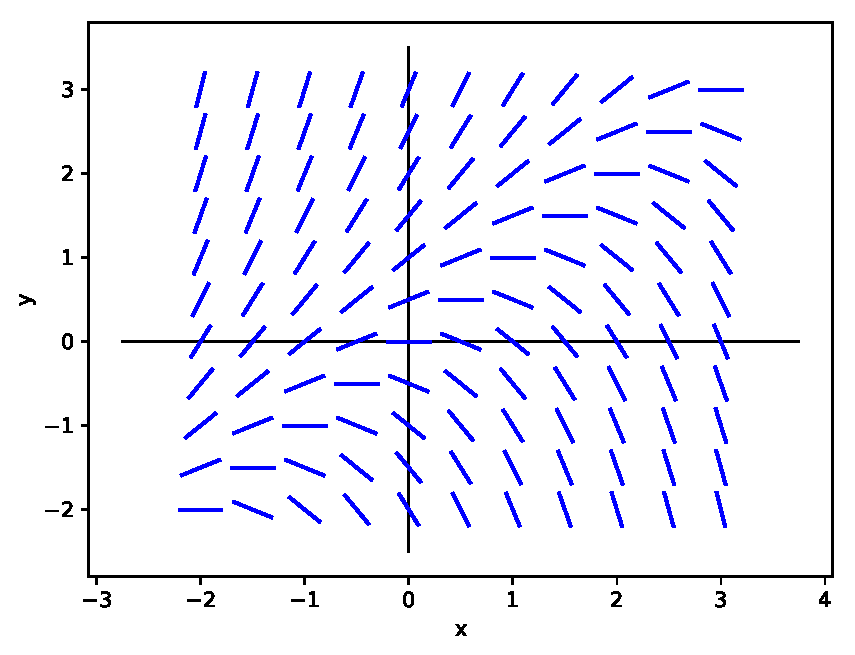
\includegraphics[width=0.9\textwidth]{figs/yminusx-dirfield}
\end{center}

\epartpts{a}{10}  Which differential equation is shown?  \circled{Circle one.}

\bigskip
\begin{center}
\begin{tabular}{ll}
A.\quad $\displaystyle \frac{dy}{dx} = 2x-1$ \hspace{35mm} & D.\quad $\displaystyle \frac{dy}{dx} = y\sin(x)$ \\
\\
B.\quad $\displaystyle \frac{dy}{dx} = y^2$ & E.\quad $\displaystyle \frac{dy}{dx} = y-x$ \\
\\
C.\quad $\displaystyle \frac{dy}{dx} = x+y$ & F.\quad $\displaystyle \frac{dy}{dx} = xy$
\end{tabular}
\end{center}

\bigskip\bigskip
\epartpts{b}{5}  Sketch on the direction field the solution $y(x)$ to the initial value problem:
    $$\frac{dy}{dx} = f(x,y), \qquad y(1)=0.$$
\underline{Label this curve as {\Large \textbf{(b)}}.}

\bigskip\bigskip
\epartpts{c}{5}  Also sketch two steps of length $h=1$ of the Euler method for solving this \emph{different} initial value problem:
    $$\frac{dy}{dx} = f(x,y), \qquad y(1)=1.$$
\underline{Label this curve as {\Large \textbf{(c)}}.}

\newpage
\probpts{4}{10}  Solve this initial value problem for a first-order linear differential equation:
    $$y' - y = -x, \qquad y(0) = 0 \hspace{100mm}$$
\vfill
\hfill $y(x) = \fbox{\LARGE \strut \hspace{60mm} \strut}$

\probpts{5}{10}  Use the definition of the Laplace transform to show that
    $$\LLL{y'(t)} = s Y(s) - y(0)$$
(Note we write $Y(s)$ for $\LLL{y(t)}$.)
\vfill

\newpage
\probpts{6}{15}  Use the Laplace transform to solve the initial value problem:
    $$y'' - y = 0, \qquad y(0) = 4, \quad y'(0)=0 \hspace{100mm}$$
\vfill
\hfill $y(t) = \fbox{\Huge \strut \hspace{60mm} \strut}$

\newpage
\probpts{7}{10}  Verify that $\displaystyle y(t)=\frac{1}{2} \left(e^t - \sin(t) - \cos(t)\right)$ solves the initial value problem:
    $$y''+y=e^t, \qquad y(0)=0, \quad y'(0)=0$$
(Do not solve the problem from scratch.  \emph{Verify} that \emph{all} parts of the IVP are satisfied.)
\vfill

\probpts{8}{10}  Write the following ODE as a first-order system:
    $$y''+y=e^t \hspace{120mm}$$
\vspace{0.75in}

\hfill \fbox{$\begin{matrix} & \\ \phantom{sdflkj} = & \phantom{sdflkj sdflkj asdf a} \\ & \\ \phantom{sdflkj} = & \\ & \end{matrix}$}

\probpts{Extra Credit I}{3}  Write several lines of \Matlab/\Octave code to solve problem \textbf{7}, at the top of this page, using \texttt{ode45}.  In particular, show how to generate the approximate value of $y(3)$.

\bigskip
\begin{Verbatim}
>>

>>

>>
\end{Verbatim}

\newpage
\probpts{9}{15}  Find and simplify the general solution of the system
    $$\bX' = \begin{pmatrix} -1 & 1 \\ 3 & 1 \end{pmatrix} \bX$$
You may use the fact that the eigenvalues and eigenvectors of $\bA=\begin{pmatrix} -1 & 1 \\ 3 & 1 \end{pmatrix}$ are
    $$\lambda_1 = -2, \quad \lambda_2=2, \qquad \bK_1 = \begin{pmatrix} 2 \\ -2 \end{pmatrix}, \quad \bK_2 = \begin{pmatrix} 1 \\ 3 \end{pmatrix}$$
\vfill
\hfill $\bX(t) = \begin{pmatrix}\, \fbox{\LARGE \strut \hspace{60mm} \strut}\, \\ 
\\
 \fbox{\LARGE \strut \hspace{60mm} \strut} \end{pmatrix} $

\bigskip
\probpts{Extra Credit II}{3}  Compute and simplify $e^{\bA t}$ if $\bA = \begin{pmatrix}
0 & 1 \\ -1 & 0 \end{pmatrix}$.  (\emph{Hint.}  Pattern in $\bA^k$?)
\vspace{2.0in}

\newpage
\prob{10}  Consider the following initial value problem:
    $$y''-y=0, \qquad y(0)=0, \quad y'(0)=2$$

\epartpts{a}{15}  Solve the problem using power series, starting from the expression $\displaystyle y(x)=\sum_{n=0}^\infty c_n x^n$.  Your solution should make it clear how $c_0$ and $c_1$ are found, and it should include a recurrence relation for the coefficients.  Find $c_0,c_1,c_2,c_3,c_4$ specifically.
\vfill

\hfill $\begin{matrix}
c_0 = \fbox{\large \strut \hspace{20mm}} \\
\\ 
c_1 = \fbox{\large \strut \hspace{20mm}} \\ 
\\
c_2 = \fbox{\large \strut \hspace{20mm}} \\ 
\\
c_3 = \fbox{\large \strut \hspace{20mm}} \\
\\
c_4 = \fbox{\large \strut \hspace{20mm}} \end{matrix} $

\bigskip
\epartpts{b}{5}  What is the radius of convergence $R$ of the power series in part \textbf{(a)}?
\vspace{0.5in}


\newpage
\begin{center}
\scriptsize
\newcommand{\dd}{\,d}
\newcommand{\dx}{\,dx}

\centerline{\textsc{Brief Table of Integrals} \hspace{30mm}}

\begin{align*}
\int x^n \dx &= \frac{1}{n+1}x^{n+1}+c, \hspace{1ex} n\neq-1 &
   \int \sec^2 x \dx &= \tan x + c \\
\int \frac{1}{x}\dx &= \ln |x| + c &
   \int \sec x \tan x \dx &= \sec x + c \\
\int u \hspace{2pt} \dd{v} &= uv - \int v du &
   \int \frac{1}{a^2+x^2}\dx &= \frac{1}{a} \arctan\left(\frac{x}{a}\right) + c \\
\int e^x \dx &= e^x + c &
   \int \frac{1}{a^2-x^2}\dx &= \frac{1}{2a}\ln\left|\frac{x+a}{x-a}\right| + c \\
\int a^x \dx &= \frac{1}{\ln a} a^x + c &
   \int \frac{1}{\sqrt{a^2-x^2}} \dx &= \arcsin\left(\frac{x}{a}\right) + c \\
\int \ln x \dx &= x \ln x - x + c &
   \int \frac{1}{x \sqrt{x^2-a^2}} \dx &= \frac{1}{a} \operatorname{arcsec}\left(\frac{x}{a}\right) + c \\
\int \sin x \dx &= -\cos x + c &
   \int \frac{1}{\sqrt{x^2-a^2}} \dx &= \ln\left|x+\sqrt{x^2-a^2}\right| + c  \\
\int \cos x \dx &= \sin x + c &
   \int \frac{1}{\sqrt{x^2+a^2}} \dx &= \ln\left|x+\sqrt{x^2+a^2}\right| + c \\
\int \tan x \dx &= \ln |\sec x| + c &
   \int \sqrt{a^2-x^2} \dx &= \frac{x}{2} \sqrt{a^2-x^2} + \frac{a^2}{2} \arcsin\left(\frac{x}{a}\right) + c \\
\int \sec x \dx &= \ln |\sec x + \tan x| + c &
   \int \sqrt{x^2+a^2} \dx &= \frac{x}{2} \sqrt{x^2+a^2} + \frac{a^2}{2} \ln\left|x+\sqrt{x^2+a^2}\right| + c
\end{align*}

\normalsize

\medskip
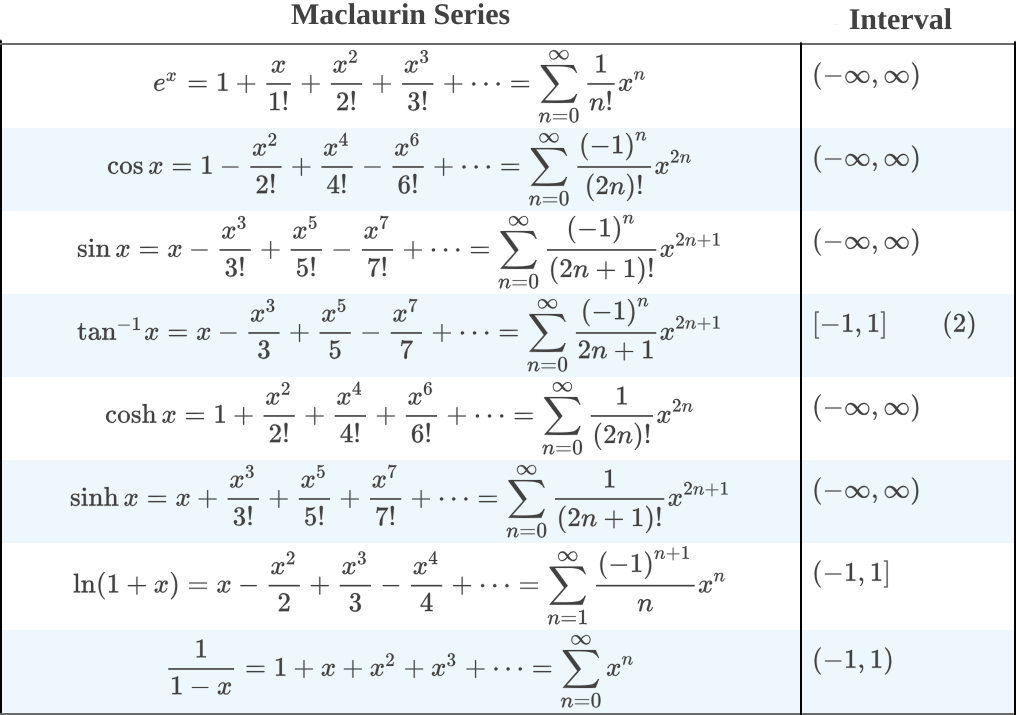
\includegraphics[width=0.7\textwidth]{figs/familiarseries}

\bigskip
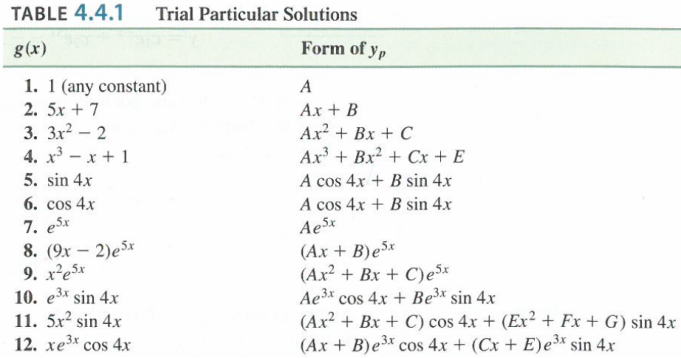
\includegraphics[width=0.64\textwidth]{figs/yptable}
\end{center}

\newpage
\textsc{Table of Laplace Transforms}:

\addtolength{\jot}{3pt}


\newcommand{\LL}[1]{\mathcal{L}\left\{#1\right\}}

\begin{minipage}[t]{0.5\textwidth}
\begin{align*}
\LL{1} &= \frac{1}{s} \\
\LL{t} &= \frac{1}{s^2} \\
\LL{t^n} &= \frac{n!}{s^{n+1}} \\
\LL{t^{-1/2}} &= \frac{\sqrt{\pi}}{s^{1/2}} \\
\LL{t^{1/2}} &= \frac{\sqrt{\pi}}{2s^{3/2}} \\
\LL{t^\alpha} &= \frac{\Gamma(\alpha+1)}{s^{\alpha+1}} \\
\LL{e^{at}} &= \frac{1}{s-a} \\
\LL{\sin(kt)} &= \frac{k}{s^2+k^2} \\
\LL{\cos(kt)} &= \frac{s}{s^2+k^2} \\
\LL{\sinh(kt)} &= \frac{k}{s^2-k^2} \\
\LL{\cosh(kt)} &= \frac{s}{s^2-k^2}
\end{align*}
\end{minipage}
\begin{minipage}[t]{0.5\textwidth}
\begin{align*}
\LL{te^{at}} &= \frac{1}{(s-a)^2} \\
\LL{t^n e^{at}} &= \frac{n!}{(s-a)^{n+1}} \\
\LL{e^{at}\sin(kt)} &= \frac{k}{(s-a)^2+k^2} \\
\LL{e^{at}\cos(kt)} &= \frac{s-a}{(s-a)^2+k^2} \\
\LL{t\sin(kt)} &= \frac{2ks}{(s^2+k^2)^2} \\
\LL{t\cos(kt)} &= \frac{s^2-k^2}{(s^2+k^2)^2} \\
\LL{e^{at}f(t)} &= F(s-a) && \\
\LL{\mathcal{U}(t-a)} &= \frac{e^{-as}}{s} \\
\LL{f(t-a) \mathcal{U}(t-a)} &= e^{-as} F(s) \\
\LL{g(t) \mathcal{U}(t-a)} &= e^{-as} \LL{g(t+a)} \\
\LL{t^n f(t)} &= (-1)^n \frac{d^n}{ds^n}F(s)
\end{align*}
\end{minipage}

\medskip
\begin{center}
\begin{minipage}[t]{0.7\textwidth}
\begin{gather*}
\LL{f^{(n)}(t)} = s^n F(s) - s^{n-1} f(0) - \dots - f^{(n-1)}(0) \\
(f\ast g)(t) = \int_0^t f(\tau)g(t-\tau)\,d\tau \\
\LL{f\ast g} = F(s) G(s)
\end{gather*}
\end{minipage}
\end{center}


\addtolength{\jot}{-3pt}

\bigskip\bigskip

\noindent \hrulefill

\footnotesize \centerline{ \textsc{space below is available for computations \hspace{30mm} clearly label anything you want graded}}
\vfill

\newpage
\footnotesize \centerline{ \textsc{space below is available for computations \hspace{30mm} clearly label anything you want graded}}
\vfill

\end{document}
